%\documentclass[wcp,gray]{jmlr} % test grayscale version
\documentclass[wcp]{jmlr}

% The following packages will be automatically loaded:
% amsmath, amssymb, natbib, graphicx, url, algorithm2e

%\usepackage{rotating}% for sideways figures and tables
%\usepackage{longtable}% for long tables

% The booktabs package is used by this sample document
% (it provides \toprule, \midrule and \bottomrule).
% Remove the next line if you don't require it.
%\usepackage{booktabs}

% The siunitx package is used by this sample document
% to align numbers in a column by their decimal point.
% Remove the next line if you don't require it.
%\usepackage[load-configurations=version-1]{siunitx} % newer version
%\usepackage{siunitx}

% The following command is just for this sample document:
%\newcommand{\cs}[1]{\texttt{\char`\\#1}}

\jmlrvolume{vol}
\jmlryear{2012}
\jmlrworkshop{ACML 2012}

\title[RRTPI]{Policy Iteration on Continuous Domains using Rapidly-exploring Random Trees}

 % Use \Name{Author Name} to specify the name.
 % If the surname contains spaces, enclose the surname
 % in braces, e.g. \Name{John {Smith Jones}} similarly
 % if the name has a "von" part, e.g \Name{Jane {de Winter}}.
 % If the first letter in the forenames is a diacritic
 % enclose the diacritic in braces, e.g. \Name{{\'E}louise Smith}

 % Two authors with the same address
  %\author{\Name{Author Name1} \Email{abc@sample.com}\and
  % \Name{Author Name2} \Email{xyz@sample.com}\\
  % \addr Address}

 % Three or more authors with the same address:
 % \author{\Name{Author Name1} \Email{an1@sample.com}\\
 %  \Name{Author Name2} \Email{an2@sample.com}\\
 %  \Name{Author Name3} \Email{an3@sample.com}\\
 %  \Name{Author Name4} \Email{an4@sample.com}\\
 %  \Name{Author Name5} \Email{an5@sample.com}\\
 %  \Name{Author Name6} \Email{an6@sample.com}\\
 %  \Name{Author Name7} \Email{an7@sample.com}\\
 %  \Name{Author Name8} \Email{an8@sample.com}\\
 %  \Name{Author Name9} \Email{an9@sample.com}\\
 %  \Name{Author Name10} \Email{an10@sample.com}\\
 %  \Name{Author Name11} \Email{an11@sample.com}\\
 %  \Name{Author Name12} \Email{an12@sample.com}\\
 %  \Name{Author Name13} \Email{an13@sample.com}\\
 %  \Name{Author Name14} \Email{an14@sample.com}\\
 %  \addr Address}


 % Authors with different addresses:


\editor{Steven C.H. Hoi and Wray Buntine}
% \editors{List of editors' names}

\begin{document}

\maketitle

\begin{abstract}
Reinforcement Learning on continuous states and continuous actions is a challenging task. Sampling based planners such as Rapidly exploring Random Trees have been widely successful in solving path planning problems. In this paper, we combine some of these planning based techniques to develop a novel policy iteration based algorithm to solve optimal control problems in continuous domains. We show that this algorithm is fundamentally sound and present experimental results on some standard domains.
\end{abstract}
\begin{keywords}
Reinforcement learning, Continuous state action, RRTs, model based
\end{keywords}

\section{Introduction}
Reinforcement Learning(RL) deals with learning optimal control strategies through interactions with the world. One of the major hindrances in applying existing RL techniques to real world scenarios, is their inability to deal with continuous state and action variables. This necessitates state abstractions when applying these techniques. A  simple and straightforward example of state abstraction is an uniform grid based discretization of the space. Such a discretization is seldom useful as a very fine grid runs into the curse of dimensionality whereas a course grid lacks sufficient representative power. To overcome this problem, variable resolution discretization techniques have been proposed \citep{munosvariablehigh,partigame}. These adopt a top-down approach where the algorithm begins with a single grid discretization and subsequently splits the space based on certain local and global heuristics. The resulting algorithms however, lack theoretical guarantees of converging to a solution that is optimal in the original continuous problem. Function approximation techniques such neural networks, support vector regression, decision trees, Gaussian processes regression, etc. maybe used to represent the value functions instead of lookup tables in the standard algorithm. Some of these techniques lack theoretical convergence guarantees and in general require careful selection of paramters.\\
In the field of robotics, large continuous domains are frequently encountered in path planning problems. Sampling based planning techniques, such as Rapidly-exploring Random Trees(RRTs) and Probabilistic Road Maps(PRMs), have been very effective in solving such problems. They possess several useful asymptotic guarantees and ability scale well to higher dimensions \citep{rrt}. However, the aim of such algorithms is limited to finding feasible paths to specified goal regions. Although there have been extensions to these algorithms that try to optimize on the quality of solution (discussed in the related work section), their main aim remains the same. In this paper, we present an novel algorithm that extends sampling based techniques, namely RRTs, to solve continuous optimal control problems. The resulting algorithm possess asymptotic convergence guarantees as well as the ability to work in continuous high dimensional domains. The space filling properties of RRTs provide an effective method of sampling the space. Our algorithm uses this set of samples to represent a partition of the space.

\section{Related work}
RRTs are simple and easy to implement planning tools that possess good scalability on higher dimensional domains. They are known to be asymptotically complete, i.e.  guaranteed to find a solution if one exists as long as the algorithm is run long enough. A recent extension of the standard RRT algorithm is RRT*, an algorithm that is capable of producing asymptotically \emph{optimal} paths while maintaining the asymptotic completeness property\citep{karaman}. The optimality of a given path is measured based on its length in the configuration space. This algorithm is said to work on a binary-cost map where, there are just obstacles and free space. It does not optimize on a arbitrarily defined reward. The idea of biasing RRTs based on a given cost map or a heuristic has been studied earlier in the continuous planning domain. In their work on heuristically biased RRTs \citep{heuristicrrt}, the authors present an algorithm that combines heuristic search techniques like the estimated cost-to-go with sampling based planning. Although they do not optimize on an arbitrary given cost and only look at reaching goal regions, ideas for biasing the RRT expansion are discussed. Transition based RRTs \citep{transrrt,gradientrrt} look to optimize paths based on a given cost by using transitions tests, similar to stochastic optimization techniques that favor more optimal paths. Different concepts of optimality itself are discussed in this work. The one that is closest to a conventional reinforcement learning is the Integral Cost. The authors on the other hand favor a minimum mechanical work criteria that seems to avoid high cost regions locally while sacrificing overall path length. In general, the aim of a conventional RL agent is to maximize the long term rewards. The reward signal is the only available feedback, and trying to optimize other local criteria might lead to distracting the agent from its global aim \citep{jettebicycle}. Our algorithm draws a lot of inspiration from these works. In a rough sense, the algorithm presented here estimates the cost (or the overall reward) of states by sampling and then grows an RRT biased according to the so evaluated \emph{value function}. This process is then carried out iteratively, similar to the policy iteration algorithm. The following section clearly defines the notion of long term reward, value functions and policy iteration.

\section{Preliminaries}
A Markov Decision Process(MDP) is described as $\left\langle S,A,T,R\right\rangle$. $S\in \mathbb{R}^n$ is the domain of states. Each state has a corresponding set of allowed actions $A_s$. This set maybe discrete or continuous. The set $A$ is defined as $\bigcup_{s} A_s $. This essentially saying, the set of actions $A$ is not characterized by labels. Performing action `1' in some state and performing the action `1' in another state does not mean the same action is performed in both states. $T$ is the state transition function $T:S \times A \rightarrow S$ .  $R$ is a real valued reward function $R:S \times A \rightarrow \mathbb{R}$. The aim of the \textit{RL agent} is to maximize the discounted cumulative reward defined as the \emph{return}, given by $ \sum_{t} \gamma^tr_t $, where $\gamma \in (0,1)$ is the discount factor.
A policy $\pi$ is a mapping from the state space $S$ to the action space $A$. $\pi :S \times A_s \rightarrow (0,1)$ that is, it represents the probability of choosing some action at a given state $s$. $J^\pi(s)$ is the state value function and is equal to the expected long term rewards, by following policy $\pi$ starting from state $s$. Similarly, $Q^\pi(s,a)$ is the state-action value function. The value function might be expressed as,
\begin{equation}
\label{eq:Vbell}
\forall s \in S,\;\; J^\pi(s) = \sum_{a}\pi(s,a)( R(s,s') + \gamma J^\pi(s'))
\end{equation}
where $s'$ is the state transitioned to according to the transition dynamics $T$. A policy $\pi^*$ is optimal if $ \forall s,\pi\;\; J^{\pi^*}(s)\geq J^\pi(s) $. The optimal value function $J^*$ can be calculated by replacing the expectation with the max operator. Since we deal with discrete dynamics, we will use denote the max as taken over all possible next states $s'$ from a given state $s$. With a slight abuse of notation we may write
\begin{equation}
\label{eq:Vopt}
\forall s \in S,\;\; J^\pi(s) = \max_{s'}( R(s,s') + \gamma J^\pi(s'))
\end{equation} 

\subsection{Approximate Policy Iteration}
\label{sec:api}
Policy Iteration is an iterative algorithm for determining the optimal policy given an MDP \citep{rlbook}. The first step is policy evaluation, which is evaluating the value function as given by \equationref{eq:Vbell}. Following which is the policy improvement step, where the policy is improved by making it greedy with respect to the value function. 
\[ \pi_{m+1}(s) = \arg_{s'} \max J^{\pi_m}(s') \]
Where $\pi_m$ corresponds to the policy evaluated in the $m^{\textit{th}}$ iteration of the algorithm. This algorithm eventually converges to a policy that is optimal. Value iteration is an algorithm, that similarly evaluates the optimal value function $J^{*}$ by turning \equationref{eq:Vopt} into an iterative update.\\
When dealing with continuous states and actions, the value function as well as the policy cannot be represented completely using tables. Thus some approximate representation is used which leads to some error. The approximation can be introduced in representing the value function and representing the policy. This framework is referred to as Approximate Policy Iteration(API). API is a fundamentally sound algorithm, meaning if the errors in the mentioned approximations are bounded, then the algorithm converges to a policy close to the optimal policy. Also as the errors decrease, the algorithm converges to the original optimal policy. The following theorem has been presented in \citep{neurodp}. 
\begin{theorem}
Let $\hat{\pi}_m$ be the policy and $J^{\hat{\pi_m}}$ be the corresponding value function approximated in the $m^{\textit{th}}$ iteration. Let $\epsilon$ and $\delta$ be the error in approximation in the value function and the policy correspondingly. If
\[ \forall m\,\, \parallel \hat{J}^{\hat{\pi}_m} - J^{\hat{\pi}_m} \parallel_{ \infty }\,\, \leq \epsilon \] and 
\[ \forall m\,\, \parallel \hat{\pi}_m - \pi_m \parallel_{ \infty } \,\,\leq \delta \]
then the final policy converges to a solution whose performance is bounded as
\[ \limsup_{m\rightarrow \infty} \parallel \hat{J}^{\hat{\pi}_m} - V^{*} \parallel_{ \infty }\,\, \leq \dfrac{\delta + 2 \gamma \epsilon}{(1-\gamma )^2} \]
\end{theorem}
We will show in the later sections that our algorithm also falls under the API framework and that it is fundamentally sound.

\subsection{Rapidly-exploring Random Trees(RRTs)}
\label{sec:rrt}
\begin{figure}[htb]
% Caption and label go in the first argument and the figure contents
% go in the second argument
\centering
\label{fig:rrt}
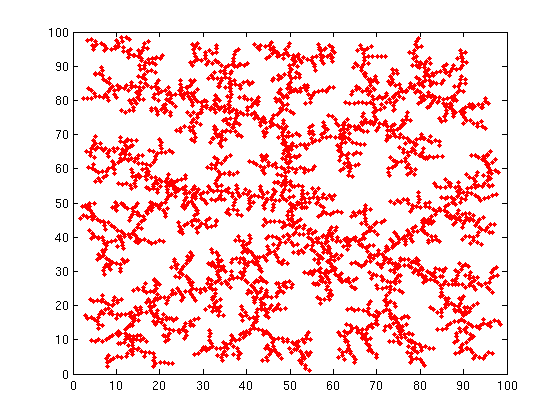
\includegraphics[scale=0.45]{rrt.png}
\caption{RRT with 300 nodes grown in $(0,100)^2$ starting from (50,50)}
\end{figure}

The basic RRT construction is outlined in \algorithmref{alg:basicrrt}. Figure 1 shows a RRT grown in a 2 dimensional space. The algorithm builds a Tree $G$ of samples from some metric space $S$ whose nodes and edges are represented by $V(G)$ and $E(G)$. The tree is rooted from a given state $s_{start}$ and is grown as described in Algorithm 1. The \texttt{Extend} routine takes two points $x$ and $y$ and returns a point $z$ such that \[ \mathcal{D}(x,y) > \mathcal{D}(z,y) \] where $\mathcal{D}$ is a distance measure defined on $S$. The feasibility of a path from x to z is also checked. The amount by which the extension can take place is limited by some parameter $\eta$. i.e. $\mathcal{D}(x,y) \leq \eta$.

\begin{algorithm2e}
\caption{ConstructRRT($s_{start},\,rrtsize$)}
\label{alg:basicrrt}
\dontprintsemicolon
$V(G)=s_{start},\,E(G)=\emptyset$\;
\Repeat{$|V(G)|=rrtsize$}{Uniformly sample a state $s_{sample}$\;
$s_{near}$ $\leftarrow$ \texttt{Nearest}($V(G),s_{sample}$)\;
$s_{ext}\leftarrow$ \texttt{Extend}($s_{near},s_{sample}$) 
$V(G) = V(G) \cup s_{ext}$\;
$E(G) = E(G) \cup (s_{near},s_{ext})$\;
}
\end{algorithm2e}
The construction of RRTs is very elegant and simple, yet they posses some interesting properties\citep{rrt} as outlined below.
\begin{theorem}
RRTs are probabilistically complete. \[ \forall{s\in S},\,\, \lim_{\textit{rrtsize} \rightarrow \infty } Pr(s \in V(G)) = 1 \]
\end{theorem}
That is, given enough time the RRT fills the space. In fact RRTs can be thought of as a online or \emph{Monte-Carlo} space filling trees. The tree is biased towards exploring new areas in the state space. It can be seen that the nodes in the graph partition the space $S$ into the corresponding Voronoi regions. When a point is sampled uniformly from the space, the probability that it falls into one of these regions and hence the probability that the corresponding node in the graph $s_{near}$ is chosen for extension is proportional to the volume of its Voronoi space.
\begin{theorem}
Probability of choosing a node $s$ to be extended is $ \dfrac{1}{\eta} \textit{Vor}(s)$
\end{theorem}
We will extend this basic RRT construction algorithm to solve optimal control problems by growing the tree in the state space of the MDP and using the samples to evaluate the value function.

\section{The Algorithms}
Given a control problem, represented as a MDP $ \mathcal{M}=$ $\left\langle S,A,T,R\right\rangle$, we present an algorithm RRT based Policy Iteration(RRTPI) that combines sampling methods such as RRTs in an iterative manner to find optimal trajectories in $\mathcal{M}$. We make the assumption that state space $S$ is metric and has some distance measure $ \mathcal{D} $ associated with it. We will first discuss a naive but intuitive algorithm, following which we will present the actual RRTPI algorithm. We begin by describing methods of generating samples and evaluating the value function based on these samples.
\subsection*{RRST}
\begin{algorithm2e}
\caption{ConstructRRST($p,rrtsize$)}
\label{alg:rrst}
\dontprintsemicolon
$V(G)=s_{start},\,E(G)=\emptyset$\;
\While{$|V(G)| \leq rrtsize$}{
$s_{sample} \sim p(S)$\;
$s_{near} \leftarrow $ \texttt{Nearest} $(s_{sample},V(G))$\;
$s_{ext} \leftarrow$ \texttt{Extend} $(s_{near},s_{sample})$\;
\If{$s_{ext} \neq \emptyset $}{
$V(G) = V(G) \cup s_{ext}$\;
$r\sim$ \texttt{SampleReward} $(s_{near},s_{ext})$\;
$E(G) = E(G) \cup (s_{near},s_{ext},r)$\;
}
}
\end{algorithm2e}
Rapidly-exploring Random Sample Trees(RRSTs), outlined in \algorithmref{alg:rrst}, is a method to grow RRT like trees in the state space of the MDP $\mathcal{M}$.  The algorithm takes as input a probability distribution function $p$ according to which random samples are generated in state space. It adds edges to the graph along with the reward $r$ corresponding to the transition. This reward information is stored in the edges of the tree.\\

In order to implement this algorithm, we make the following two assumptions:
\begin{enumerate}
\item The algorithm needs access to a generative model of the world. This model allows us to sample the reward for arbitrary transitions.
\item A local approximate controller. This corresponds to the \texttt{Extend} subroutine. Given a starting state and a direction(denoted by a target state), the controller tries to generate feasible actions that leads to a state as defined in the \sectionref{sec:rrt}. This assumption is similar to the local greedy controller assumption used in the parti-game algorithm \citep{partigame}.
\end{enumerate}

\subsection*{Evaluating the Value function}
\begin{figure}[htb]
\centering
\label{fig:rrst}
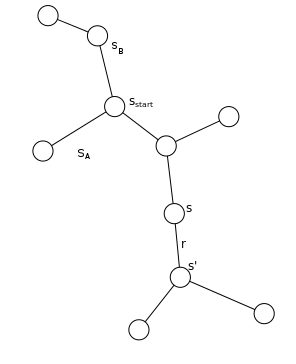
\includegraphics[scale=0.4]{rrst.png}
\caption{A small RRST. This corresponds to a discretization of the original MDP.}
\end{figure}

The RRST algorithm generates generates a tree in the state space of MDP $\mathcal{M}$ as shown in Figure 2. The state space can be discretized into partitions corresponding to the Voronoi regions of the nodes of the tree. The set of edges represent the possible transitions. Thus the process of growing the RRST corresponds to discretization of the state and action space of the given MDP $\mathcal{M}$. We can now define a discretized MDP whose states are represented by $V(G)$ and actions are represented by $E(G)$. We then describe a policy $\pi^{rrt}(s,s') \varpropto Vor(s')$ where $\pi(s,s')$ is the probability of choosing the edge between $s$ and $s'$ $Vor(s')$ is the volume of the Voronoi region of state $s$. Thus for eg. in Figure 2,
\begin{equation*}
\frac{\pi^{rrt}(s_{start},s_A)}{\pi^{rrt}(s_{start},s_B)} = \frac{Vor(A)}{Vor(B)}
\end{equation*}
We can now evaluate the corresponding value function $J^{rrt}$ by solving the bellman equations described in \equationref{eq:Vbell}.
This can be done using iterative policy evaluation.
\begin{equation}
\label{eq:poleval}
\forall s \in V(G),\;\; J^{rrt}(s) = \sum_{s'}\pi(s,s')( R(s,s') + \gamma J^{rrt}(s'))
\end{equation}\\
We then generalize the value function $J^{rrt}$ to the original MDP $\mathcal{M}$ by defining it as 
\begin{equation*}
\forall s \in S,\;\; \hat{J}(s) = J^{rrt}(s_{near})
\end{equation*}
where $s_{near}$ is \texttt{Nearest}($s,V(G)$). i.e. a piecewise constant approximation with the basis as the set of states defined in $V(G)$.
\subsection*{Naive RRTPI}
We can now describe a simple algorithm that is similar to the policy iteration procedure.\\
\begin{enumerate}
\item Construct a RRST initially using uniform random distribution
\item Evaluate the value function as described in \equationref{eq:poleval}
\item Bias the probability distribution $p(s) \varpropto \hat{J}(s)$  and construct the RRST
\item Repeat steps 2 and 3 iteratively till convergence
\end{enumerate}
Intuitively, step 2 of the algorithm corresponds to policy improvement, while step 3 corresponds to policy evaluation. This algorithm however does not perform as expected in practice. A closer look reveals some of the shortcomings of this naive algorithm. We discuss them and motivate the steps of the final RRTPI algorithm.

\begin{itemize} 
\item Constructing a pdf from the Value function is non-trivial and requires some sort of bin or particle set approximation. This pulls the tree towards the globally optimal nodes, even through potentially low value nodes. Thus this step cannot be shown to correspond exactly with the  policy improvement step. The value function incorporates the long term goodness of moving to a particular state and a policy that is locally greedy w.r.t to its own value function is indeed optimal \citep{rlbook}. So, the node to which the transition is made to - $s_{ext}$, must be chosen maximally based on its value $J(s_{ext})$.  

\item In order to evaluate $\pi(s,s')$ the volume of the Voronoi region of nodes must be computed. The original RRT algorithm, does this implicitly and biases the exploration proportionally to the volume of the Voronoi region. We modify the algorithm based on ideas from the Heuristic RRTs \citep{heuristicrrt} and use rejection sampling in the \texttt{Extend} subroutine to only select new states with sufficiently good value. We can directly compute the optimal value function $J_{rrt}^*(s)$ corresponding to \equationref{eq:Vopt} instead. Thus we have
\begin{equation}
\label{eq:polmax}
\forall s \in V(G),\;\; J_{rrt}^*(s) = \max_{s'}( R(s,s') + \gamma J_{rrt}^*(s'))
\end{equation}
This can be done using the value iteration algorithm.


\item Some MDPs are of finite horizon (such as the mountain car problem). Growing the particular branch of the tree must be stopped after the corresponding termination condition in the original condition has been reached. The leaves of the tree that have not reached the termination condition might lead to an incorrect value function, as during the evaluation step, these are considered as terminal states(since they have no further next states). Thus the tree must be pruned to contain only branches that have terminated. This may impose the condition that the tree has to be grown until at least one branch reaches termination which may require a very long time. The scarcity of rewards is a problem RL in general. RRTs are particularly suited in this case because, they posses excellent space filling properties and occupy space at an exponential rate.

\begin{figure}[htb]
\centering
\label{fig:case}
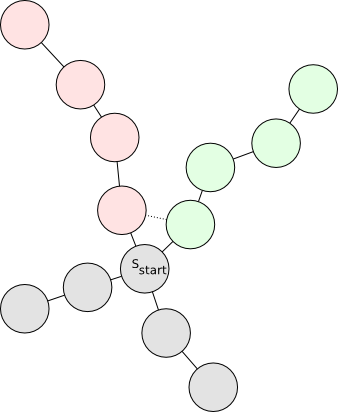
\includegraphics[scale=0.45]{case.png}
\caption{States in the green branch of the tree have high value, whereas the ones on the red branch have low value. The value between the states marked by dotted line is not generalized well even when it is possible to connect them using the controller. }
\end{figure}

\begin{figure}[htb]
\centering
\label{fig:rrg}
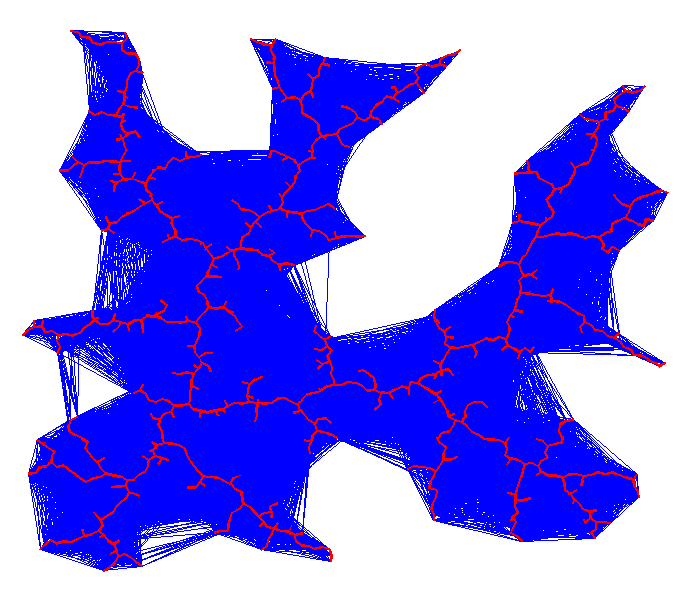
\includegraphics[scale=0.45]{rrg.png}
\caption{Forming a DAG instead of a Tree. The DAG is shown in blue, the corresponding the Tree is shown in red.}
\end{figure}


\item Consider the case where there are two branches of the tree that are very close to each other in distance as shown in Figure 3. One reaches a highly rewarding state, whereas the other does not. Thus the value backed up by the value iteration algorithm will be dramatically different along the states in the branch. Although these states are close to each-other distance wise, their value is poorly generalized. There may have been a critical decision in the history of the two branches that leads to this disparity, although we observe that this is not the case as there can be many valid transitions between the nodes of the two branches. This was observed to be true in the continuous grid world domain. This seems to hint that growing a directed acyclic graph(DAG) instead of a tree might lead to better generalization. This is similar to the asymptotically optimal path planning technique RRT* \citep{karaman}. In fact this is related to the fact that the plain RRT algorithm can be proved to be non-optimal for path planning \citep{karaman}. Constructing such a DAG is shown in \algorithmref{alg:rrsg}. We use the parameter $\eta$ that defines the extent of the local controller. Connections are attempted between all nodes in the graph that are within an $\eta$-radius of $s_{ext}$ to $s_{ext}$, where $s_{ext}$ is the new node being added to the DAG. Successful connections are added to the edge set and the corresponding rewards are stored as well. An example of such a DAG constructed in a 2 dimensional space is shown in Figure 4. Constructing a DAG involves some additional work, but as shown, the extra edges improve the quality of solution. $\eta$ maybe be chosen to decrease, as the number of nodes in the graph increase. Typically, choosing $\eta$ to be proportional to $dfrac{n}{\log n}$ results in the addition of $O(\log n)$ edges per node, and thus the number of edges increase to $O(n\log n)$ compared to $O(n)$ for the tree. 

\end{itemize}

\begin{algorithm2e}
\caption{ConstructRRSG($p,rrtsize$)}
\label{alg:rrsg}
\dontprintsemicolon
$V(G)=s_{start},\,E(G)=\emptyset$\;
\While{$|V(G)| \leq rrtsize$}
{
	$s_{sample} \leftarrow$ \texttt{Sample} ($p$)\;
	$s_{near} \leftarrow $ \texttt{Nearest} $(s_{sample},V(G))$\;
	$s_{ext} \leftarrow$ \texttt{Extend} $(s_{near},s_{sample})$\;
	$S_{\eta} \leftarrow$ $\eta$-\texttt{Near} $(s_{ext},V(G))$\;
	$V(G) = V(G) \cup s_{ext}$\;
	\For{valid $s' \in S_{\eta} \cup s_{near} $}
	{		
		$r\sim$ \texttt{SampleReward} $(s',s_{ext})$\;
		$E(G) = E(G) \cup (s',s_{ext},r)$\;
	}
}
\end{algorithm2e}



\subsection*{RRTPI}
The RRTPI algorithm is presented in \algorithmref{alg:rrtpi}. This incorporates solutions to all issues discussed above. At any time in the construction of the DAG, the new node to be added $s_{ext}$ is chosen according to its value. This is achieved by first scaling $\hat{J}$ to $(0,1)$ and using rejection sampling. The value function $\hat{J}$ itself is learned by evaluating the optimal value function $J_{rrt}^*$ in the discretized MDP and then generalizing it as a piecewise constant function. Thus by iteratively evaluating and improving the policy, the algorithm eventually converges to a optimal trajectory.  Convergence can be determined by checking if the change in the average value of the nodes along the optimal path of the graph is within some bound.\\
Figure 5 shows the algorithm finding a near optimal path in a simple 2 dimensional continuous gridworld. The controller corresponds to straight line paths within some distance. The reward function is -1 everywhere and on reaching the goal, the termination flag is raised along with a reward of +100. Hitting obstacles or the boundary gives a reward of -10 and the episode terminates. The value function that is learnt is shown in Figure 6. In the next section we will show some properties of this algorithm and then finally present results on standard benchmarks comparing the RRTPI algorithm with other algorithms.

\begin{figure}[htb]
\centering
\label{fig:iter1}
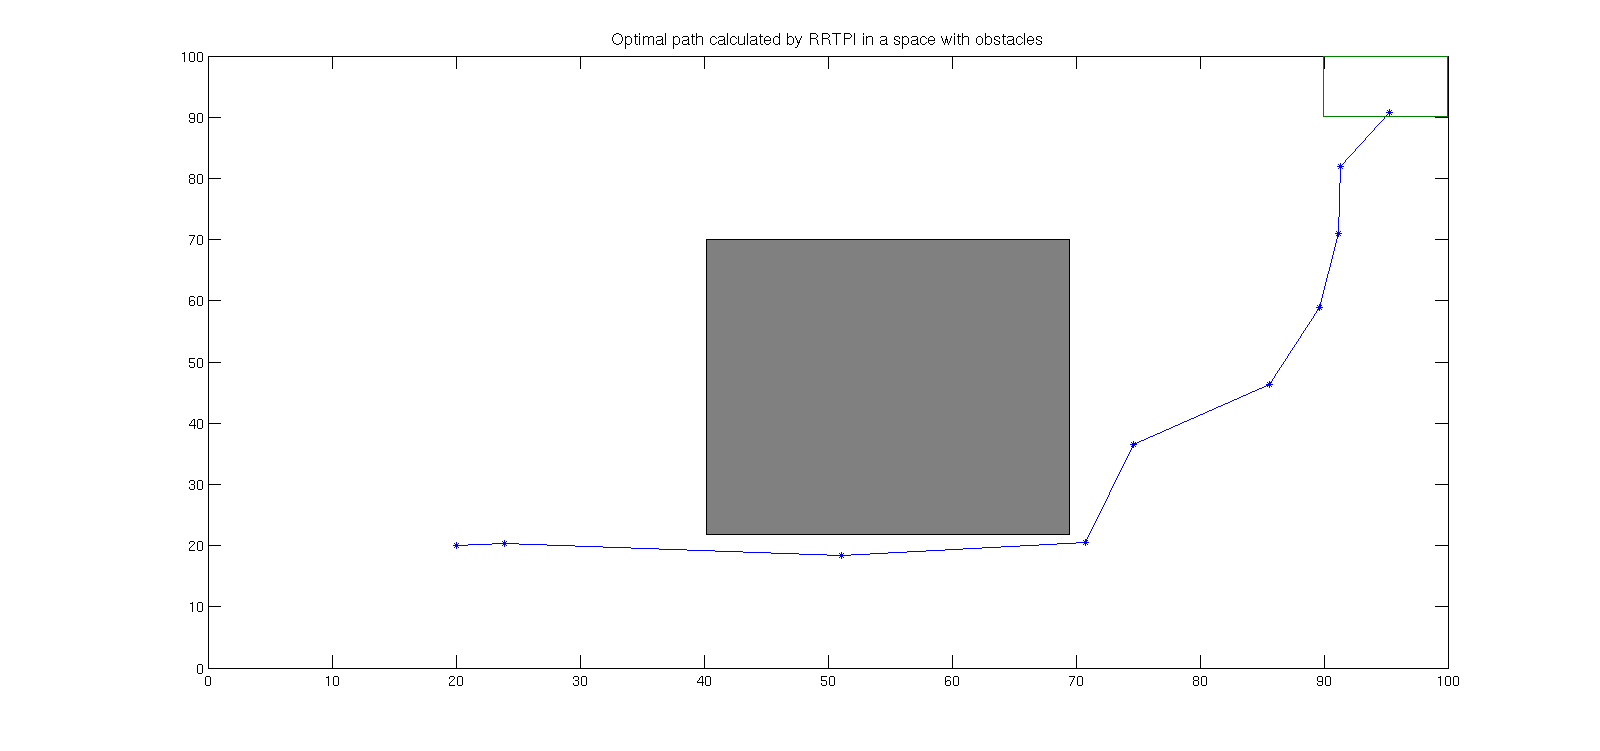
\includegraphics[width=420px]{rrtpi1.png}
\caption{RRTPI solving a 2 dimensional gridworld. The gray region is an obstacle and the green box represents the goal regions.}
\end{figure}

\begin{figure}[htb]
\centering
\label{fig:val1}
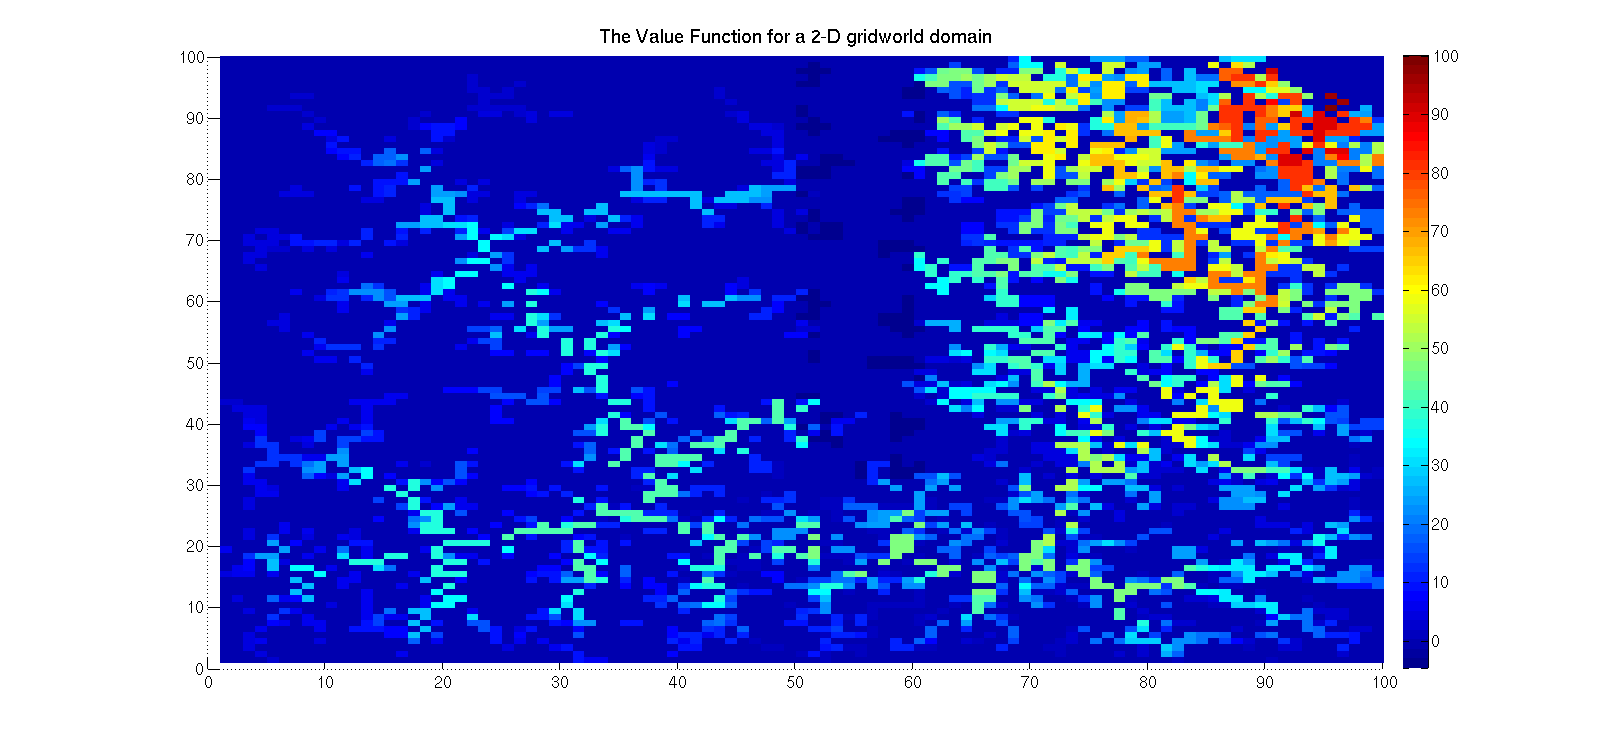
\includegraphics[width=450px]{valufunction.png}
\caption{Heat map showing the value function learnt on the state space of the gridworld MDP}
\end{figure}

\begin{algorithm2e}
\caption{RRTPI($rrtsize$)}
\label{alg:rrtpi}
\dontprintsemicolon
Initialize $ \forall s \hat{J}(s) \leftarrow 0$\;
\Repeat{convergence}
{
	$V(G)=s_{start},\,E(G)=\emptyset$\;
	\While{$|V(G)| \leq rrtsize$}
	{
		$s_{sample} \leftarrow$ Sample uniformly from $S$\;
		$s_{near} \leftarrow $ \texttt{Nearest} $(s_{sample},V(G))$\;
		$s_{ext} \leftarrow$ \texttt{Extend} $(s_{near},s_{sample})$\;
		\If{$\hat{J}(s_{ext}) < rand(0,1)$}
		{
		$continue$\;
		}
		$S_{\epsilon} \leftarrow$ $\epsilon$-Near $(s_{ext},V(G))$\;
		$V(G) = V(G) \cup s_{ext}$\;
		\For{valid $s' \in S_{\epsilon} \cup s_{near} $}
		{		
			$r\sim$ \texttt{SampleReward} $(s',s_{ext})$\;
			$E(G) = E(G) \cup (s',s_{ext},r)$\;
		}	
	}
$solve\;\;\forall s \in V(G),\;\; J_{rrt}^*(s) = \max_{s'}( R(s,s') + \gamma J_{rrt}^*(s'))$\;
$\forall s \in S,\;\; \hat{J}(s) = J^{rrt}(s_{nearest})$ where $s_{nearest} =$ Nearest$(s,V(G))$ \;
\texttt{Scale} $\hat{J}$ to $[0,1]$
}
\end{algorithm2e}

\section{Discussions}
 We present some results on the RRTPI algorithm.\\
\begin{figure}[htb]
\centering
\label{fig:val1}
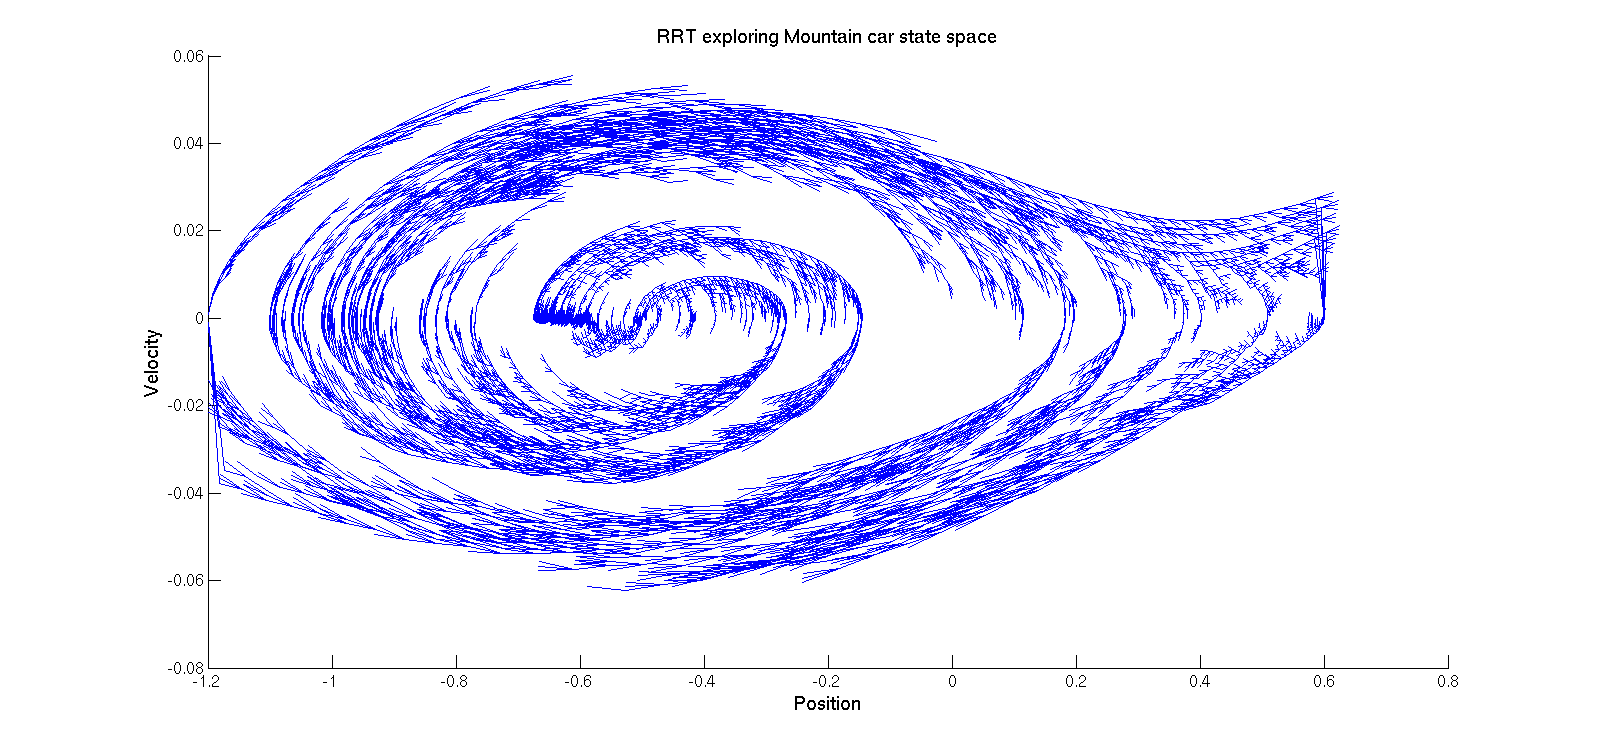
\includegraphics[width=450px]{rggpi.png}
\caption{The first iteration of the rrtpi algorithm on the mountain car domain}
\end{figure}

By construction it can be seen that the DAG version has all the properties of the RRT algorithm discussed in \sectionref{sec:rrt}. Namely asymptotic completeness and bias towards larger Voronoi regions.
\begin{theorem}
RRTPI is a fundamentally sound algorithm.
\end{theorem}
\begin{proof}
We will prove the theorem by adapting the generic proof of Approximate Policy Iteration as shown in \sectionref{sec:api}. It suffices to show that the error in approximating the policy as well as the value function is bounded. \\
We first show that the constructing the graph implicitly corresponds to policy improvement. The probability of forming an edge between $s_{ext}$ and $s_{near}$ is given by 
\[ Pr(\text{Choosing }s_{near}) \times Pr(\text{Choosing }s_{ext}) \]
\[ \varpropto Vor(s_{near})\times \hat{J}(s_{ext}) \] and $\hat{J}$ corresponds to the optimal value function of the discretized MDP represented by the Graph.

The construction of the graph possesses properties similar to RRTs. Thus,\\
\[ \lim_{rrtsize \rightarrow \infty } Pr(s\in V(T)) \rightarrow 1\,\,, \forall s\in S \] 
The sampling graph constructed in the RRTPI algorithm discretizes the given MDP $\mathcal{M}=\left\langle S,A,T,R \right\rangle $ into a discrete MDP $\mathcal{M'}=\left\langle V(G),E(G),T',R \right\rangle $ By construction of the graph and the asymptotic completeness property,
\[ \lim_{rrtsize \rightarrow \infty } V(G) \rightarrow S \]
\[ \lim_{rrtsize \rightarrow \infty } E(G) \rightarrow A \]
If $J^*$ is the optimal value function corresponding to the original MDP and $\hat{J}$ is the value function described in RRTPI algorithm then from the above result it follows that
\[  \forall s \in S,\;\; \lim_{rrtsize \rightarrow \infty } |J^*(s)- \hat{J}(s) | \rightarrow 0 \]
Thus the error in approximating the value function can be trivially bound as there exists some $rrtsize$ for which the above error is within a given bound $\epsilon$. The policy is implicitly represented using the value function itself. Thus we can conclude that the algorithm fits into the API framework and hence is fundamentally sound.\\

 The main issue with forming a DAG as mentioned above, is that connecting two arbitrary states in the space might be a difficult task. This is especially true in the case of under-actuated systems, where it may sometimes even be impossible to do so. For some under actuated domains such as the mountain car, we do not construct a DAG but instead use the same RRRTPI described above with a tree,  omitting the part where connections are made to other existing nodes in the graph. Such a tree is shown in Figure 7. This algorithm still converges to good solutions as can be seen in experimental results section.
\end{proof}


\section{Experimental results}
The performance of the algorithm was first evaluated in a simple continuous grid world as shown in the previous section. The algorithm produces policies that are similiar to the optimal paths produced my the RRT* algorithm. The algorithm was also compared with Q learning on a uniform discritized grid and an adaptive resolution technique presented in \citep{munosvariablehigh}. The comparison is performed on a standard 2 dimensional domain, the mountain-car. The domain is described in \citep{mcar}. The results are summarized in Figure 8. The RRTPI algorithm is run with a limit on the number of nodes in the graph. The algorithm shows close to optimal performance on this domain with a relatively low number of states. The performance measure is the average return of the initial state, averaged across 50 runs.\\
Next we compare the performance on the acrobot domain. The domain used here is described in Chapter 11 of \cite{rlbook}. The results are summarized in Figure 9. As can be seen the RRTPI algorithm is again able to generate good solutions with relatively smaller number of samples.

\begin{figure}[htb]
\centering
\label{fig:res1}
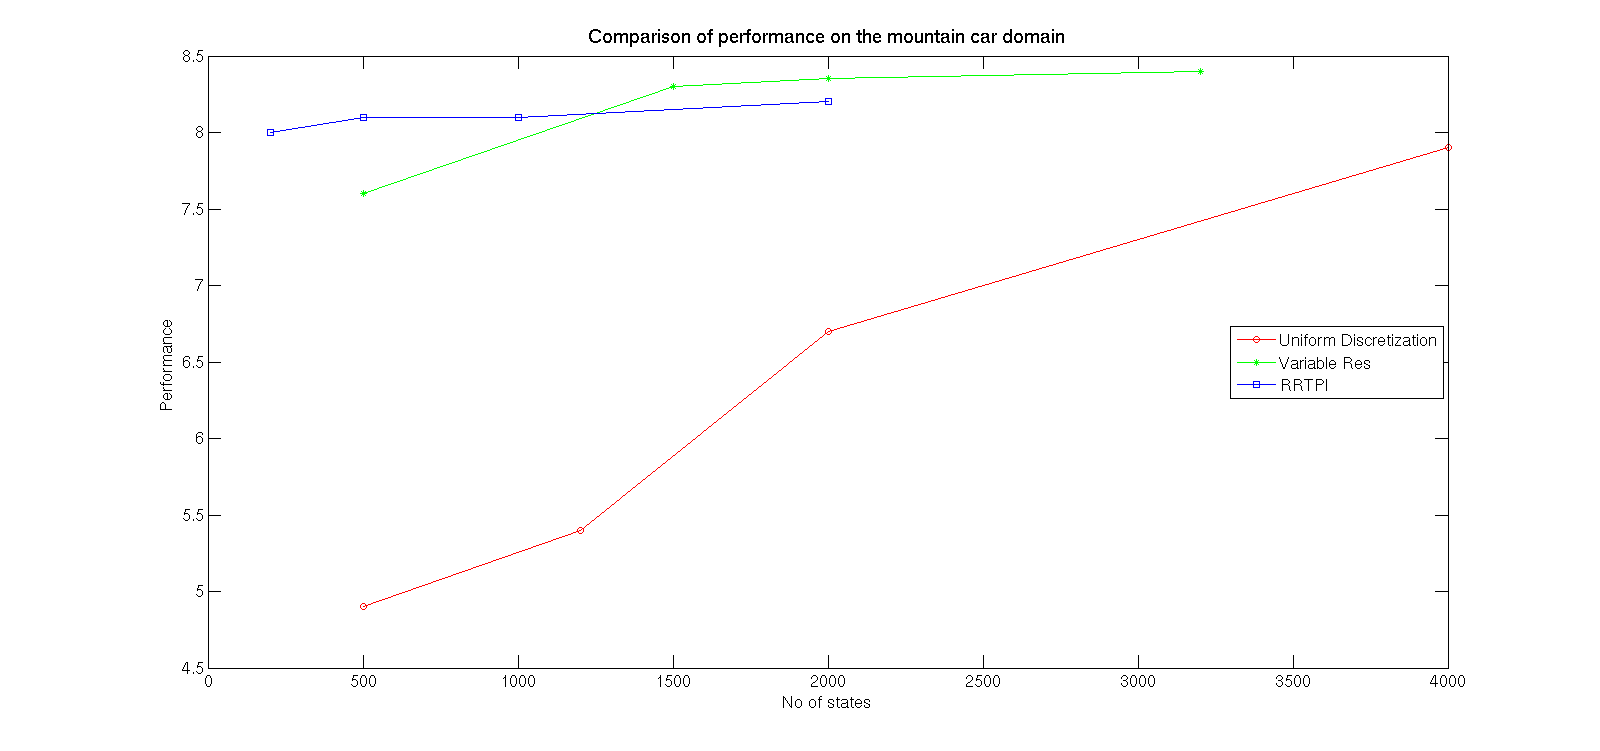
\includegraphics[scale=0.33]{res1.png}
\caption{RRTPI performs competitively on the standard mountain car domain}
\end{figure}

\begin{figure}[htb]
\centering
\label{fig:res2}
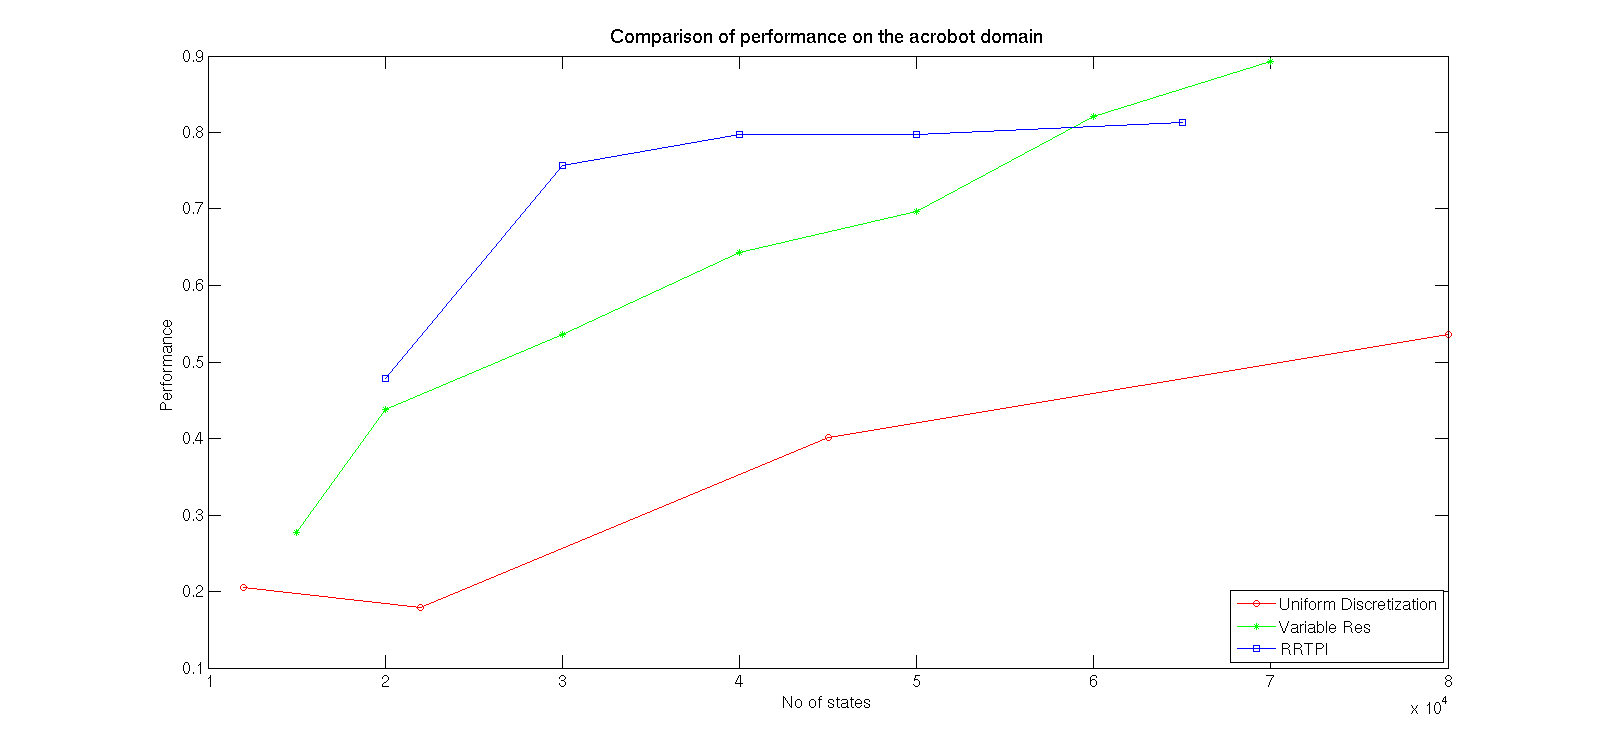
\includegraphics[scale=0.33]{res2.png}
\caption{RRTPI performs competitively on the standard mountain car domain}
\end{figure}


\section{Conclusion and Future Work}
We present RRTPI, a novel algorithm that combines the properties of sampling based continuous domain planners to solve problems of optimal control. This algorithm is shown to have competitive performance in standard domains.  The algorithm has been proved to be asymptotically complete and fundamentally sound.  Further interesting analysis, can be carried out on the rate of convergence and the sample complexity. By using some of the properties of Random Geometric Graphs as discussed for the RRT* algorithm \citep{karaman}, we may be able to prove that the graph constructed possesses fast mixing properties. Thus providing a starting point for arriving at results on sample complexity and rate of convergence. 

\bibliography{rrtpi1}


\end{document}
